\documentclass[paper=a4, fontsize=11pt]{scrartcl} % A4 paper and 11pt font size

\usepackage{float}
\usepackage{graphicx}
\usepackage{hyperref}
\usepackage[T1]{fontenc} % Use 8-bit encoding that has 256 glyphs
\usepackage{fourier} % Use the Adobe Utopia font for the document - comment this line to return to the LaTeX default
\usepackage[english]{babel} % English language/hyphenation
\usepackage{amsmath,amsfonts,amsthm} % Math packages

\usepackage{lipsum} % Used for inserting dummy 'Lorem ipsum' text into the template

\usepackage{sectsty} % Allows customizing section commands
\allsectionsfont{\centering \normalfont\scshape} % Make all sections centered, the default font and small caps

\usepackage{fancyhdr} % Custom headers and footers
\pagestyle{fancyplain} % Makes all pages in the document conform to the custom headers and footers
\fancyhead{} % No page header - if you want one, create it in the same way as the footers below
\fancyfoot[L]{} % Empty left footer
\fancyfoot[C]{} % Empty center footer
\fancyfoot[R]{\thepage} % Page numbefring for right footer
\renewcommand{\headrulewidth}{0pt} % Remove header underlines
\renewcommand{\footrulewidth}{0pt} % Remove footer underlines
\setlength{\headheight}{13.6pt} % Customize the height of the header

\numberwithin{equation}{section} % Number equations within sections (i.e. 1.1, 1.2, 2.1, 2.2 instead of 1, 2, 3, 4)
\numberwithin{figure}{section} % Number figures within sections (i.e. 1.1, 1.2, 2.1, 2.2 instead of 1, 2, 3, 4)
\numberwithin{table}{section} % Number tables within sections (i.e. 1.1, 1.2, 2.1, 2.2 instead of 1, 2, 3, 4)

\setlength\parindent{0pt} % Removes all indentation from paragraphs - comment this line for an assignment with lots of text

%----------------------------------------------------------------------------------------
%	PHYTN SECTION
%-

\usepackage{color}
\usepackage{listings}
\usepackage{setspace}
\definecolor{Code}{rgb}{0,0,0}
\definecolor{Decorators}{rgb}{0.5,0.5,0.5}
\definecolor{Numbers}{rgb}{0.5,0,0}
\definecolor{MatchingBrackets}{rgb}{0.25,0.5,0.5}
\definecolor{Keywords}{rgb}{0,0,1}
\definecolor{self}{rgb}{0,0,0}
\definecolor{Strings}{rgb}{0,0.63,0}
\definecolor{Comments}{rgb}{0,0.63,1}
\definecolor{Backquotes}{rgb}{0,0,0}
\definecolor{Classname}{rgb}{0,0,0}
\definecolor{FunctionName}{rgb}{0,0,0}
\definecolor{Operators}{rgb}{0,0,0}
\definecolor{Background}{rgb}{0.98,0.98,0.98}
\lstdefinelanguage{Python}{
numbers=left,
numberstyle=\footnotesize,
numbersep=1em,
xleftmargin=1em,
framextopmargin=2em,
framexbottommargin=2em,
showspaces=false,
showtabs=false,
showstringspaces=false,
frame=l,
tabsize=4,
% Basic
basicstyle=\ttfamily\small\setstretch{1},
backgroundcolor=\color{Background},
% Comments
commentstyle=\color{Comments}\slshape,
% Strings
stringstyle=\color{Strings},
morecomment=[s][\color{Strings}]{"""}{"""},
morecomment=[s][\color{Strings}]{'''}{'''},
% keywords
morekeywords={import,from,class,def,for,while,if,is,in,elif,else,not,and,or,print,break,continue,return,True,False,None,access,as,,del,except,exec,finally,global,import,lambda,pass,print,raise,try,assert},
keywordstyle={\color{Keywords}\bfseries},
% additional keywords
morekeywords={[2]@invariant,pylab,numpy,np,scipy},
keywordstyle={[2]\color{Decorators}\slshape},
emph={self},
emphstyle={\color{self}\slshape},
%
}
%----------------------------------------------------------------------------------------
%	TITLE SECTION
%----------------------------------------------------------------------------------------

\newcommand{\horrule}[1]{\rule{\linewidth}{#1}} % Create horizontal rule command with 1 argument of height

\title{	
\normalfont \normalsize 
\textsc{Middle East Technical University, CENG 776} \\ [25pt] % Your university, school and/or department name(s)
\horrule{0.5pt} \\[0.4cm] % Thin top horizontal rule
\huge Efficient set intersection for inverted indexing paper report \\ % The assignment title
\horrule{2pt} \\[0.5cm] % Thick bottom horizontal rule
}

\author{Ozgur GUNDOGAN \\ Burak Sefa SERT} % Your name


\date{\normalsize\today} % Today's date or a custom date

\begin{document}

\maketitle % Print the title

%----------------------------------------------------------------------------------------
%	PROBLEM 1
%----------------------------------------------------------------------------------------

\section{INTRODUCTION}

A conjunctive query q is equivalent to a |q|-way intersection which uses ordered sets of integers, where each set represents the documents containing one of the terms, and each integer in each set is an ordinal document identifier. Therefore, there is a tension between the way in which the data is represented, and the ways in which it is to be manipulated. In this paper, this tension tradeoffs are explored by investigating different intersection techniques. Also, author of this paper proposes a new simple hybrid method to make intersection computation faster.

\section{ALGORITHMS FOR EFFICIENT F-SEARCH}
\paragraph{}
To intersect two or more lists , we need to search the items in other lists. Also, finger search (F-Search) step is the an important part of an intersection process as computationally.  In this part , we will discover different type of f-search algorithms.
\paragraph{}
Although binary search is not so efficient search algorithm, it is used in other search algorithms. That's why it is needed to be mentioned here with an example. 
To examplify binary search, let's think about two ordered sets S and T , with |S| = s  and  |T| = t, and $s \leq t$ . Binary search over t elements requires $1+\log t$ comparisons. In particular, binary search is the optimal approach when s = 1.

\paragraph{}
There are also other searching methods linear search, interpolation search, Fibonacci search, exponential search and Golomb search. The desirable characteristic of these alternatives is that the search cost grows as a function of the distance traversed, rather than the size of the array. For example, linear search requires O(d) time to move the finger by d items; exponential search requires $O(\log d)$ time.

\paragraph{}
In situations when $1 \ll  n_{1} \ll  n_{2} $, use of exponential search is considerable benefit. In an exponential search, probes into T are made at exponentially increasing rank distance from the current location, until a value greater than the search key is encountered. A binary search is then carried out within the identified subrange. In this approach each F-SEARCH call requires $1+2* \log d$ comparisons, where d is the difference between the rank of the finger's previous position and the new rank of the finger pointer. 

\paragraph{}
Golomb searching also can be used.Progressively, search proceeds is similar to exponential search, but with a fixed forwards step of b items used at each iteration, not exponentially increasing. Once overshoot has been achieved, a binary search takes place over the (lastly) b items that have been identified . When searching through a set of size $n_{2}$ for the elements of a set of size $n_{1}$, the correct value for the step b is 0.69(n2/n1), with a total search cost that is again proportional to O($n_{1}$ + $n_{1}$ $\log$($n_{2}$/$n_{1}$)).

Golomb and binary search are implemented in python. It can be seen here.

\section{Intersection Methods}

\subsection{Binary Intersection of Ordered Sets}
In binary Intersection of ordered sets, we intersect two lists one by one. Progressively,
each element of the smaller set, S, is tested against the larger set, T , and retained if it is present. The search retains state as it proceeds, with the eliminator element, x, stepped through the elements of S; and the F SEARCH (finger search) operation used in T to leapfrog over whole subsequences, pausing only at one corresponding value in T for each item in S. 


\subsection{Small versus Small}

When more than two sets are being intersected, the simplest approach is to iteratively apply the standard two-set intersection method using as a sequence of pairwise operations.Small versus small (svs) approach is based on this idea. Progressively, the smallest set is identified, and then that set is intersected with each of the others, in increasing order of size. The svs method is simple and effective, and benefits from the spatial locality inherent from processing the sets two at a time. Even so, each different F-SEARCH implementation gives rise to a different svs computation.

\subsection{Adaptive Holistic Intersection}
The alternative to the svs approach is to combine all of the sets using a single sweep through them all. The resultant holistic algorithms offer the possibility of being adaptive to the particular data arrangement present. The simplest holistic approach is to treat each item in the smallest set as an eliminator, and search for it in each of the remaining sets. Conceptually, this method is identical to an interleaved version of svs.

In adaptive holistic intersection (adp), the sets are initially monotonically increasing in size. At each iteration, the eliminator is the next remaining item from the set with the fewest remaining elements. If a mismatch occurs before all sets have been examined, the sets are reordered based on the number of unexamined items remaining in each set, and the successor from the smallest remaining subset becomes the new eliminator. This approach reduces the number of item-to-item comparisons expected to be required, but at the possibly non-trivial cost of reordering the |q| lists at each iteration of the main loop.

\subsection{Sequential Holistic Intersection}

In sequential holistic intersection (seq) , algorithm uses as the next eliminator the element that caused the previous eliminator to be discarded, and continues the strict rotation among the sets from that point. Only when an eliminator value is found in all the sets – and hence is part of the intersection's output – is a new eliminator chosen from the smallest set. This approach has the advantage that the sets do not need to be reordered, while still allowing all of the sets to provide eliminators. However, this method suffers from a practical disadvantage: more F-SEARCH operations are likely to accrue when the eliminator is drawn from a populous set than when it is drawn from one of the sparse sets in the intersection.

\subsection{Max Successor Intersection}

Holistic methods may have a memory access pattern that is less localized than do svs methods, because all of the sets are processed concurrently. To diminish this risk, author of the paper propose a further alternative. The eliminator is initially drawn from the smallest set. When a mismatch occurs, the next eliminator is the larger of the mismatched value and the successor from the smallest set. Processing starts in $S_{2}$ if the eliminator is again taken from $S_{1}$, otherwise processing begins in $S_{1}$. The intuition behind this approach is two-fold. The first is that, without any other information, the best eliminator will be in the smallest set. The second intuition is that, having discovered a bigger than anticipated jump in one of the sets, that value should be tested against the first set, to see if additional items can be discarded.

\newpage
\section{DATASET}
The dataset we have used includes more than 500000 words and 41000000 posting list entry. It is quite big, therefore instead of importing the whole list into memory we have lazy loaded the posting list data as needed. Apart from that, query that we have used is extracted from as title of query topics, with punctuation omitted. The remaining part is split by whitespace and each word is AND'ed.


\newpage
\section{EXPERIMENTS AND RESULTS}
Throughout this project, we have implemented four methods which are small versus small, adaptive holistic intersection, sequential holistic intersection, max successor intersection. As search function, we used golomb search in max successor intersection algorithm and binary search in the rest of algorithms. Since our dataset consists queries upto 5 words in a query,  we needed to concatenate queries randomly to generate queries more than 5 words. Thanks to that, we compared methods' efficiencies with respect to query length in a better way. As can be seen in Figure \ref{fig:result_normal}, small versus small is the worst algorithm and adaptive holistic intersection algorithm is the best one in average. It can be said that the performance of the algorithms are highly query dependent if we compare query length 4 and 5. Result in query length 4 and 5 show us the adaptive holistic intersection algorithm is better than max successor when query length is 4 but worse than max successor when query length is 5. Also, if we examine result of any of algorithms in \ref{fig:result_normal}, we can see that algorithms performance do not decrease when query length increases as expected. Actually it makes sense if we think about one word query which has a long posting list and three words query which all words have a short posting list.
 


\begin{figure}[H]
   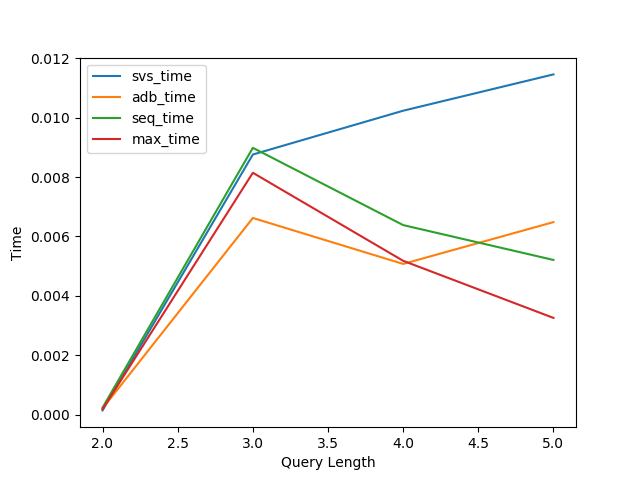
\includegraphics[width=\textwidth]{result_}
  \caption{ Original queries upto 5 words in a query}
  \label{fig:result_normal}
\end{figure}


All observations in \ref{fig:result_normal} which mentioned above are still valid for \ref{fig:result_50}. In this graph, we easily observe that some queries consume so much time with respect to others.


\begin{figure}[H]
   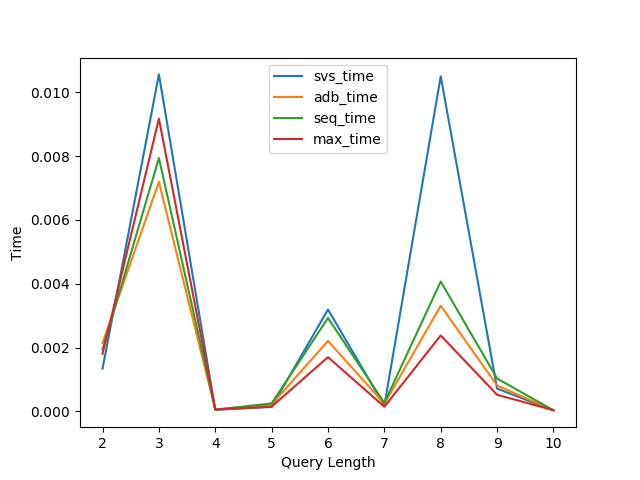
\includegraphics[width=\textwidth]{result_50}
  \caption{ Concatenated queries upto 10 words in a query}
  \label{fig:result_50}
\end{figure}



\section{CONCLUSION}
By using the results for our dataset, we can not say that one of the algorithms is better than others. Adaptive holistic intersection and max successor intersection algorithms work slightly better than others. However, performance of these two algorithms can not be comparable. We  can suggest using a combined version of these two algorithms with respect to queries which they work well.


\newpage
\section{SOURCE CODE}

All source code can be found under  \href{https://github.com/ozgurgundogan/Efficient-set-intersection-for-inverted-indexing}{Github Repository.}


\subsection{Intersection Algorithms Implementation}
\lstinputlisting[language=Python]{main/Intersections.py}

\newpage
\subsection{Search Algorithms Implementation}
\lstinputlisting[language=Python]{main/Searchs.py}



\end{document}